\documentclass[11pt]{beamer}
%\usetheme{Dresden}%{Berkeley}
\usetheme{metropolis} 
\usepackage[utf8]{inputenc}
\usepackage[english]{babel}
\usepackage{amsmath}
\usepackage{amsfonts}
\usepackage{amssymb}
\usepackage{graphicx}
\usepackage{wrapfig}
%\usepackage[font=scriptsize,labelfont=bf]{subcaption}
%\usepackage[font=scriptsize,labelfont=bf]{caption}
\usepackage{FiraSans}
\usepackage{FiraMono}

\usepackage{pgfpages}

\usepackage{lmodern}

\usepackage[binary-units = true]{siunitx}

% externalize tikz images
\usepackage{tikz}							% externalize tikz images
\usepackage{pgfplots} 					% create plots with pgf/tikz
\pgfplotsset{compat=1.14} 			% README here http://pgfplots.sourceforge.net/pgfplots.pdf
	%\usepgfplotslibrary{external}
	\usetikzlibrary{external}			%
	
	\makeatletter
	\newcommand*{\overlaynumber}{\number\beamer@slideinframe}
	\tikzset{
	  beamer externalizing/.style={%
	    execute at end picture={%
	      \tikzifexternalizing{%
	        \ifbeamer@anotherslide
	        \pgfexternalstorecommand{\string\global\string\beamer@anotherslidetrue}%
	        \fi
	      }{}%
	    }%
	  },
	  external/optimize=false
	}
	\let\orig@tikzsetnextfilename=\tikzsetnextfilename
	\renewcommand\tikzsetnextfilename[1]{\orig@tikzsetnextfilename{#1-\overlaynumber}}
	\makeatother
	
	\tikzset{every picture/.style={beamer externalizing}}	
	
	\tikzexternalize								% activate!
	\tikzsetexternalprefix{tikz/}	% set subfolder
	
\usepgfplotslibrary{fillbetween,dateplot} % need this to fill between functions
\usetikzlibrary{	patterns, decorations, decorations.markings, decorations.pathreplacing,
								shapes, shapes.geometric, shapes.misc, arrows, arrows.meta,
								positioning, intersections,
								overlay-beamer-styles,
								mindmap,trees,shadows}

\usepackage[
  backend     = biber,
  style       = phys,
  autocite    = superscript,
  sortcites   = true,
]{biblatex}
\addbibresource{../tex/bib_articles.bib}
\addbibresource{../tex/bib_books.bib}
\addbibresource{../tex/bib_websites.bib}
\usepackage{csquotes}
\renewcommand{\footnotesize}{\tiny}%{\scriptsize}
%\setbeamerfont{bibliography entry note}{size=\tiny}
%\renewcommand*{\bibfont}{\scriptsize}
%\setbeamertemplate{bibliography item}{\insertbiblabel}

\setbeameroption{show notes on second screen}

\author[D. Bazzanella]{Davide Bazzanella}
\title[All-Optical Neural Networks]{Optical Bistability As Neural Network Nonlinear Activation Function}
%\subtitle[short subtitle]{long subtitle}
%\logo{
\includegraphics[height=2.3cm]{pics/unitn_logo.png} } 
\institute[UNITN]{Università degli studi di Trento} 
\date{20th March 2018} 
\subject{Master Thesis in Physics}

\setbeamercovered{transparent} 
\setbeamertemplate{navigation symbols}{} 

\metroset{numbering=fraction, background=light}

%\newcommand{\frameofframes}{/}
%\newcommand{\setframeofframes}[1]{\renewcommand{\frameofframes}{#1}}
%\setframeofframes{of}

%\setbeamertemplate{footline}{
%	\begin{beamercolorbox}[ht=2.5ex, dp=1.125ex, leftskip=.3cm, rightskip=.3cm plus1fil]
%		{title in head/foot}
%		{\insertshorttitle} \hfill {\insertframenumber~\frameofframes~\inserttotalframenumber}
%%		{author in head/foot}
%%		{\insertshortauthor} \hfill {\insertinstitute}
%	\end{beamercolorbox}
%}

% set automatic fade transition
\addtobeamertemplate{background canvas}{\transfade}{}

% \section[Text]{Long Text}: Long Text is used in TOC, Text in navigation.
% \footfullcite{ <citation> }

\begin{document}

\frame{\titlepage}
%%%%% %%%%% %%%%% %%%%% %%%%% %%%%%
\section[Introduction]{Introduction}
\begin{frame}{All-optical Artificial Neural Networks}
	Applying integrated photonics to artificial neural networks architecture design
	
	Develop simulations on standard software libraries that help performance comparisons
\end{frame}

%%%%% %%%%% %%%%% %%%%% %%%%% %%%%%
\begin{frame}{Outline}
\tableofcontents[pausesections]
\end{frame}

%%%%% %%%%% %%%%% %%%%% %%%%% %%%%%
\section{Artificial Neural Networks}
%
\begin{frame}{ANNs}
	Artificial Neural Networks are computation systems, composed by a collection of nodes that work seemingly biological neurons.
\end{frame}
%
\begin{frame}{ANNs blocks}
	ANNs are composed by single units, \textit{nodes}, which elaborate the information in a way loosely similar to biological neurons.
	\begin{figure}
		\centering
		\tikzsetexternalprefix{tikz/}	% set subfolder
\tikzsetnextfilename{node}
\begin{tikzpicture}[baseline, scale=1]
	\node [shape=circle, minimum size=2cm, draw=gray!100, fill=gray!20]%
				(af) at (1.5,0) {\LARGE $f_a$};
	\node (aftext) [below, align=center] at (af.south) {activation \\ function};
	\node [regular polygon, regular polygon sides=6, minimum size=2cm, draw=gray!100, fill=gray!20]%
				(ws) at (-2,0) {\LARGE $\Sigma$};
	\draw (aftext.north)++(-3.5,0) node (wstext) [below, align=center] {weighted \\ sum};
	\draw (ws) to (af);
	\foreach \i in {1,2,4}	\draw (-4.5,1.5-0.6*\i) .. controls (-3.5,1.5-0.6*\i) .. (ws);
	\foreach \i in {1,2}		\node at (-4.5,1.5-0.6*\i) [left] {$x_\i$};
	\node (xn) at (-4.5,-0.9)  [left] {$x_n$};
	\draw [dashed] (-4.5,-0.3) .. controls (-3.5,-0.3) .. (ws);
	\node at (-4.5, -0.2) {$\vdots\qquad$};
	\draw (-2,1.5) node [above] {$w_0$} to (ws);
	\draw (af) to (3.5,0) node [right] {$y$};
\end{tikzpicture}
	\end{figure}
\end{frame}
%
%\begin{frame}[standout]
%	What can they do?
%\end{frame}
\begin{frame}[c]{What can they do?}
	\center \huge What can they do?
\end{frame}
%
\begin{frame}{What can they do?}
	\begin{columns}
		\column{0.6\textwidth}
			ANNs can solve complex problems:
			\begin{itemize}
				\item \alert<2>{\textbf<2>{classification}}
				\item \alert<3>{\textbf<3>{clustering}}
				\item \alert<4>{\textbf<4>{pattern recognition}}
				\item \alert<5>{\textbf<5>{time series prediction}}
			\end{itemize}
		\column{0.35\textwidth}
			\begin{figure}
				\centering
				\only<2>{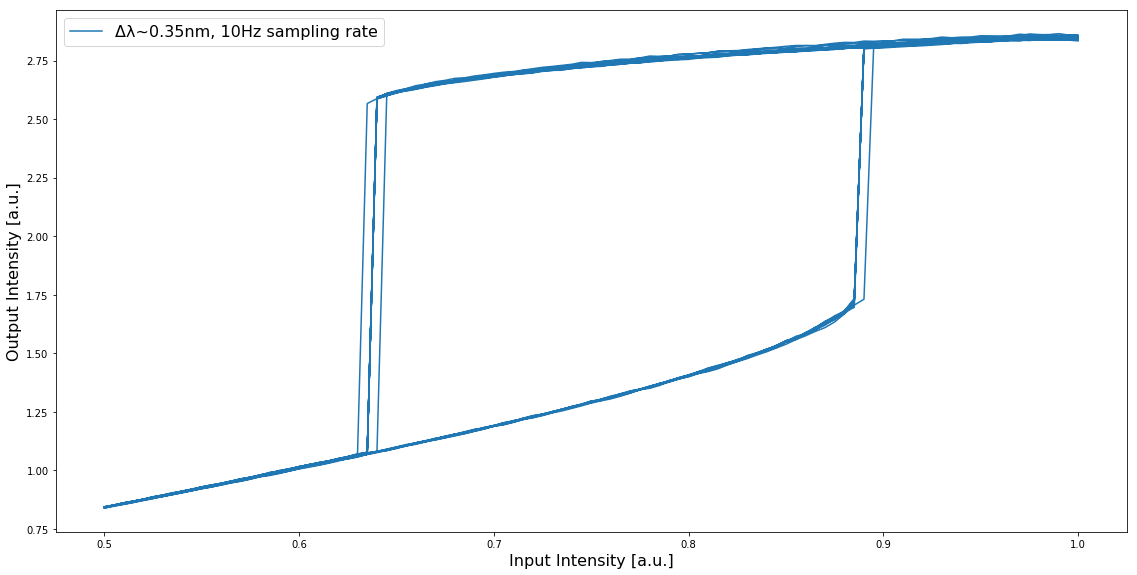
\includegraphics[draft,width=3cm,height=2cm]{figures/foo.png}}
				\only<3>{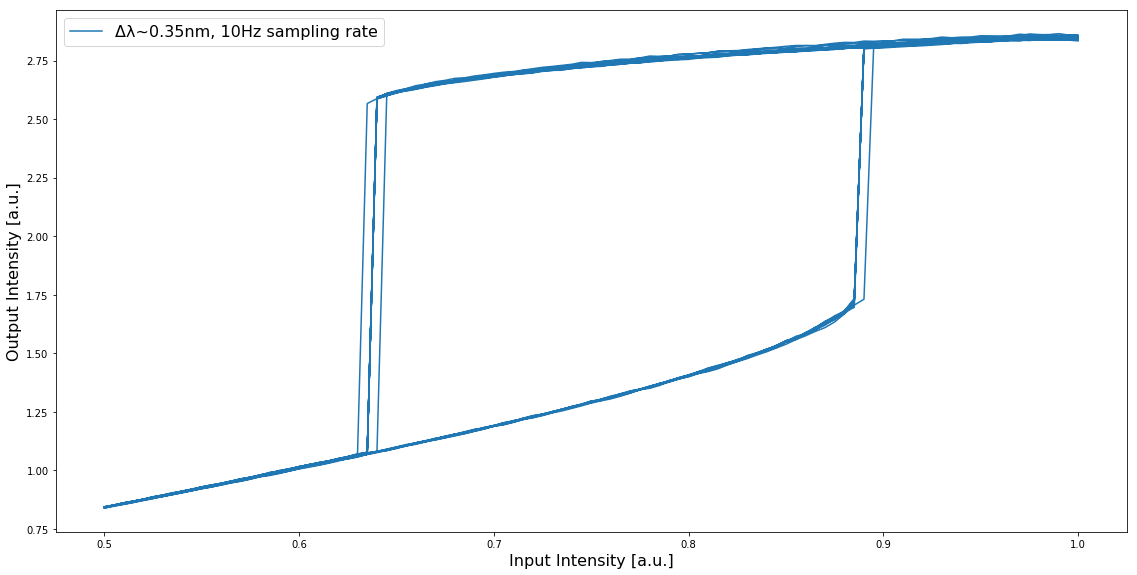
\includegraphics[draft,width=3cm,height=3cm]{figures/foo.png}}
				\only<4>{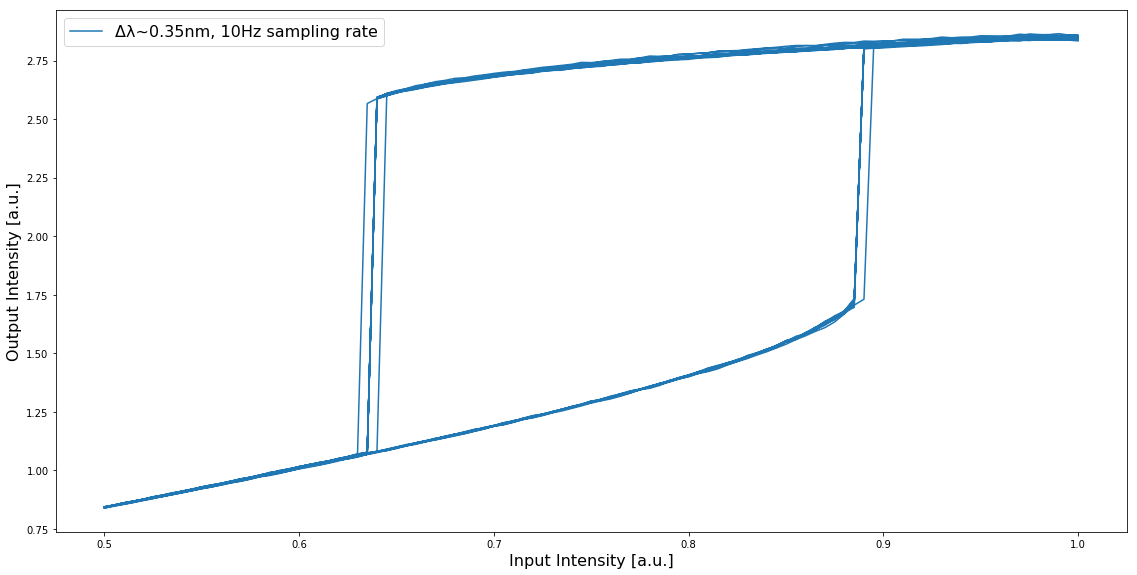
\includegraphics[draft,width=3cm,height=4cm]{figures/foo.png}}
				\only<5>{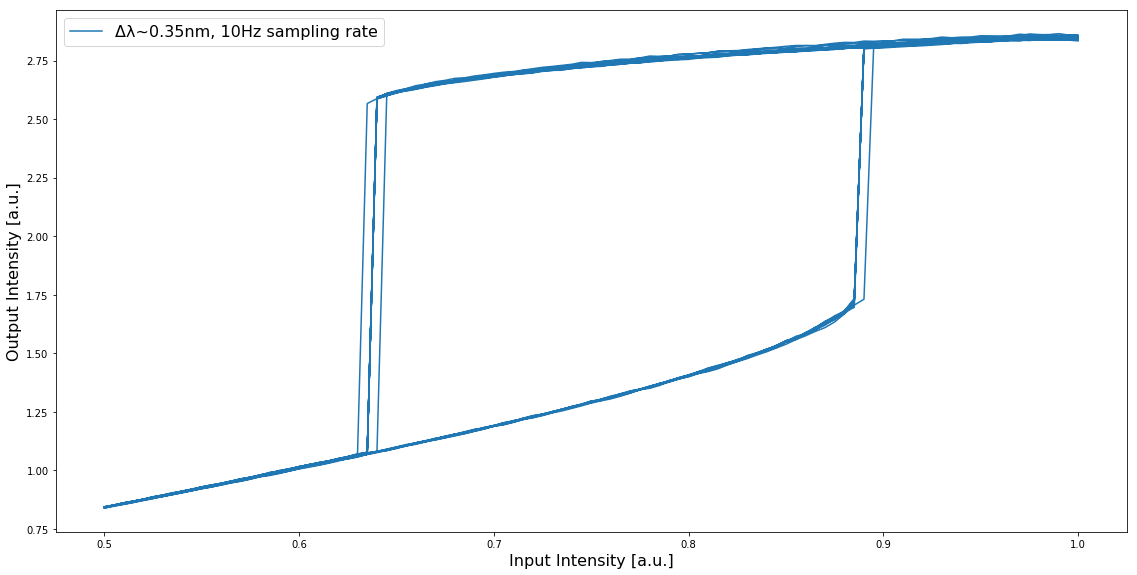
\includegraphics[draft,width=3cm,height=5cm]{figures/foo.png}}
			\end{figure}
	\end{columns}
\end{frame}
%
\begin{frame}[c]{How do they work?}
	\center \huge How do they work?
	
	\tikzset{external/export next=false}
	\begin{tikzpicture}[remember picture, overlay]
    \draw [line width=10mm, opacity=.25] (current page.center)++(-\textwidth/4,0) circle [radius=2cm];
    \node (c) at (current page.center) {};
%    \draw [->, very thick,red,opacity=0.5] (c) to[bend right] (current page.south east);
%    \draw [overlay , ->, very thick,red,opacity=0.5] (c) to[bend right] (n1);
		%\node [rotate=60,scale=2,text opacity=0.2] at (current page.center) {Example};
	\end{tikzpicture}
\end{frame}
%\begin{frame}{How do they work?}
%	ANNs can obtain arbitrary decision regions\footnotemark
%	
%	\vspace*{2em}
%	The amount of free parameters in an ANN, allow ..
%	\footnotetext{\fullcite{duda2012pattern}}%\footfullcite{duda2012pattern}
%\end{frame}
\begin{frame}{How do they work?}
	ANNs can obtain arbitrary decision regions\footnotemark
	
	\vspace*{2em}
	The amount of free parameters in an ANN, allow ..
	\tikzset{external/export next=false}\tikz[remember picture] \node [circle,fill=red!50] (n1) {};
	?
	\footnotetext{\fullcite{duda2012pattern}}%\footfullcite{duda2012pattern}
	
	\tikzset{external/export next=false}\tikz[remember picture,overlay] \draw [->, very thick,red,opacity=0.5] (c)++(-\textwidth,0) to[bend right] (n1);
\end{frame}
\begin{frame}{How do they work?}
	\begin{itemize}[<+->]
		\item training
		\begin{itemize}
			\item evaluate loss
			\item adjust parameters
		\end{itemize}
		\item validation
		\item test
	\end{itemize}
\end{frame}
%

%%%%% %%%%% %%%%% %%%%% %%%%% %%%%%
\section{Microring Resonator}
\begin{frame}{MRR}
	\begin{columns}
		\column{0.45\textwidth}
		Consider a MRR in the \textit{Add-Drop Filter} configuration
		\begin{align*}
			\texttt{T} \left( \omega \right) &= f \left[ ~\texttt{I} \left( \omega \right) ~\right] \\
			\texttt{D} \left( \omega \right) &= f \left[ ~\texttt{I} \left( \omega \right) ~\right]
		\end{align*}
		
		\visible<3->{Coupling is governed by
		\[\tau \quad \mathrm{and} \quad \kappa.\]}
		\column{0.45\textwidth}
		\begin{figure}
			\centering
			\tikzsetexternalprefix{tikz/}	% set subfolder
\tikzsetnextfilename{MRR}
\begin{tikzpicture}[
		baseline,
		scale=0.3,
		every pin edge/.style={-},
	]

%	\draw [help lines] (-3,-3) grid (3,3);
	
	\filldraw [draw=black!50, fill=gray!20, even odd rule]
		(0,0) circle [radius=4.43, thick]
		(0,0) circle [radius=4.91, thick];
	\path [name path=inner] (0,0) circle [radius=5.085];
	\path [name path=outer] (0,0) circle [radius=5.505];
%	%distance between waveguides is 9.848
	\path [name path=leftwg]  (-4.924,-6) rectangle (-5.344,+6);
	\path [name path=rightwg] (+4.924,-6) rectangle (+5.344,+6);
	
	\path [name intersections={of=inner and leftwg, name=leftyin}];
	\path [name intersections={of=outer and leftwg, name=leftyout}];
	
	\path [name intersections={of=inner and rightwg, name=rightyin}];
	\path [name intersections={of=outer and rightwg, name=rightyout}];
	
	\draw [black!50, line join=round, rounded corners=1pt, fill=gray!20]
		(-4.924,-6) -- (-5.344,-6) -- (leftyout-4)
		.. controls ++(+103:1) and ++(-103:1) .. (leftyout-2)
		-- (-5.344,+6) -- (-4.924,+6) -- (leftyin-1)
		.. controls ++(-102:1) and ++(+102:1) .. (leftyin-2)
		-- cycle;
	
	\draw [black!50, line join=round, rounded corners=1pt, fill=gray!20]
		(+4.924,-6) -- (+5.344,-6) -- (rightyout-4)
		.. controls ++(+77:1) and ++(-77:1) .. (rightyout-2)
		-- (+5.344,+6) -- (+4.924,+6) -- (rightyin-1)
		.. controls ++(-78:1) and ++(+78:1) .. (rightyin-2)
		-- cycle;
	
	\draw [semithick, -stealth] (+6.0,-6) -- (+6.0,-5) node [midway, right] {\texttt{A}};
	\draw [semithick, -stealth] (+6.0,+5) -- (+6.0,+6) node [midway, right] {\texttt{D}};
	\draw [semithick, -stealth] (-6.0,-5) -- (-6.0,-6) node [midway, left] {\texttt{T}};
	\draw [semithick, -stealth] (-6.0,+6) -- (-6.0,+5) node [midway, left] {\texttt{I}};
	
	\draw [-stealth, visible on=<1->] (0,0) -- ++(60:4.43) node [left, midway] {$R_{in}$};
				
	\draw [|-|, black, visible on=<2->] (+0,+4.430) -- (+0,+4.910) node [pin=+90:\scriptsize\SI{0.48 }{\um}] {};
	\draw [|-|, black, visible on=<3->] (+4.924,-5) -- (+5.344,-5) node [pin=200:\scriptsize\SI{0.42 }{\um}] {};
	\draw [|-|, black, visible on=<3->] (-4.924,+0) -- (-5.085,+0) node [pin=340:\scriptsize\SI{0.175}{\um}] {};

\end{tikzpicture}
%			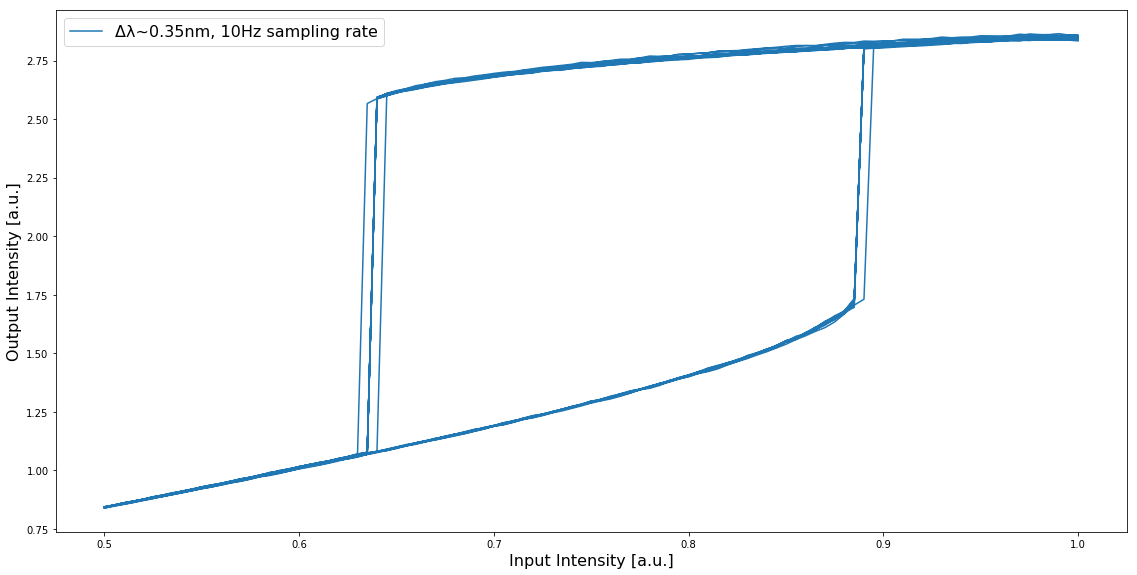
\includegraphics[draft,width=4.5cm,height=3cm]{figures/foo.png}
		\end{figure}
	\end{columns}
\end{frame}
\begin{frame}{Theory}
Linear
\end{frame}
\begin{frame}{Theory}
Nonlinear
\end{frame}
\begin{frame}[plain]{Experiments}
	\begin{figure}[htbp]
	\tikzsetnextfilename{pump_setup}

% Define size/space
\def\loopsize{.8cm}
\def\loopoffset{0.2cm}
% Define the loops
\def\myloops#1#2{
\begin{scope}[shift={#1}, scale=#2]
        % Draw the baseline
    \draw (-\loopoffset,0) -- (\loopoffset,0);
        % Draw the loops
    \draw (-\loopoffset,0)	node [draw, thick, circle, anchor=south, minimum size=\loopsize] (id) {};
    \draw (0,0) 						node [draw, thick, circle, anchor=south, minimum size=\loopsize] (id) {};
    \draw (\loopoffset,0) 	node [draw, thick, circle, anchor=south, minimum size=\loopsize] (id) {};
\end{scope}
}

\begin{tikzpicture}
	[
	source/.style ={
		draw, rectangle, inner sep=6pt, anchor=west
		},
	VOA/.style ={
		draw, circle, inner sep=2pt, fill=white, anchor=west
		},
	sample/.style={
		draw, chamfered rectangle, chamfered rectangle=8pt, anchor=west
		},
	coupler/.style={
		draw, rounded rectangle, rounded rectangle right arc=none, anchor=west, inner sep=2pt
		},
	thick,
	] %radius=5, inner sep=0pt,	minimum size=3mm}
	
	\draw (0,0) node [source, align=center] (tunics)
									{\small TUNICS\\\tiny + \\\small EYDFA}
					node [above] at (tunics.north) {source}
					node [below] at (tunics.south) {amplified}
				(tunics.east)
%				++(0.6, 0) node [source] (eydfa) {EYDFA}
%					node [above] at (eydfa.north) {amplifier}
%				(eydfa.east)
				++(0.6, 0) node [VOA] (circ) {$\scriptstyle\circlearrowright$}
%					node [above] at (circ.north) {circ}
			  (circ.east)
				++(0.6, 0) node [coupler] (couplerA) {\tiny(a)}
					node [above] at (couplerA.north east) {\tiny .5}
					node [below] at (couplerA.south east) {\tiny .5}
			   +(1.0,-1.2) node [source] (osa) {OSA}
					node [below] at (osa.south) {detector}
				(couplerA.east)
				++(1.2, 0) node (polarizer) {}
				++(1.2, 0) node [coupler] (couplerB) {\tiny(b)}
					node [above] at (couplerB.north east) {\tiny .9}
					node [below] at (couplerB.south east) {\tiny .1}
				(couplerB.east)
				++(1.0, 0) node [VOA] (voa) {$\scriptstyle\nearrow$}
					node [above] at (voa.north) {voa}
			   +(0.0,-1.2) node [source] (detectorB) {Ge B}
					node [below] at (detectorB.south) {detector}
			  (voa.east)
				++(0.6, 0) node [sample] (sample) {sample}
				(sample.east)
				++(0.6, 0) node [source] (detectorA) {Ge A}
					node [above] at (detectorA.north) {detector};
	
	\myloops{(polarizer)}{1}
	\node [below] at (polarizer) {polarizer};

	\draw (tunics) -- ++(circ) node [pos=.85, above] {\tiny (1)}
				(circ) -- (couplerA) node [pos=.15, above] {\tiny (2)}
				(circ) to [out=225, in=90] ++(-0.4,-0.6) node [circle, inner sep=1pt, black, fill=black] {}
																								node [below] {\tiny (3)}
				(circ) to [out=315, in=90] ++(+0.4,-0.6) node [circle, inner sep=1pt, black, fill=black] {}
																								node [below] {\tiny (4)}
				(couplerA.20) to [out=0, in=180] (polarizer)
				(couplerA.-20) to [out=0, in=180] (osa)
				(polarizer) to (couplerB)
				(couplerB.20) to [out=0, in=180] (voa)
				(couplerB.-20) to [out=0, in=180] (detectorB)
				(voa) -- (sample)
				(sample) -- (detectorA)
				;

\end{tikzpicture}
	\end{figure}
\end{frame}

%%%%% %%%%% %%%%% %%%%% %%%%% %%%%%
\section{ANN Simulations}
\begin{frame}{Simulation Framework}
What means simulating?
PyTorch library
\end{frame}
\begin{frame}{Fundamental blocks}
	model ($FF[f_a]$)
	
	loss criteria (CEL)
	
	weight update criteria (SGD)
\end{frame}
\begin{frame}
	model ($FF[f_a]$)
\end{frame}
\begin{frame}
	\textit{Cross-Entropy Loss} (also known as negative log likelihood),
	\begin{equation*}
		L(y, \hat{y}) = f_{CEL}(y, \hat{y}) = - \frac{1}{N} \sum_{n=1}^N \sum_{i=1}^C y_{n,i} \log \left( \hat{y}_{n,i} \right)
	\end{equation*}
\end{frame}
\begin{frame}
	\textit{Stochastic Gradient Descent}
	
	 with \textit{momentum}
	 
	 and \textit{learning rate scheduler}.
\end{frame}
\begin{frame}{Operation Tests}
ReLU vs $f_{fit}$
\end{frame}

%%%%% %%%%% %%%%% %%%%% %%%%% %%%%%
\section{Conclusion}
\begin{frame}{Overview}

	{I assembled an experimental setup from scratch}
	
	\vspace{1em}
	{I characterized the response of the MRR in several aspects}
	
	\vspace{1em}
	{I implemented the bistable response in standard software libraries}
\end{frame}
\begin{frame}{Future Perspectives}
	\visible<1->{Continue the current work with a quantitative analysis of specific features}
	
	\vspace{1em}
	\visible<2->{Enhance the physical theory to describe time dependent phenomena}
	
	\vspace{1em}
	\visible<3->{Proceed with the development of the simulations to include all the characteristics of the physical system}
%	Proceed with the implementation of physical characteristics in the simulations
\end{frame}

%\section[]{References}
%\begin{frame}[allowframebreaks]{References}
%\printbibliography
%\end{frame}

\begin{frame}{Mindmap}
\tikzsetexternalprefix{tikz/}	% set subfolder
\tikzsetnextfilename{mindmap}
\begin{tikzpicture}[mindmap, concept color=gray!50!violet, font=\sf, text=white]

  \tikzstyle{level 1 concept}+=[font=\sf, sibling angle=90,level distance = 30mm]

  \node[concept,scale=0.7] {Center}
    [clockwise from={90+45}]
        child[concept color=red, visible on=<2->]{ node[concept,scale=0.7]{NW} } 
        child[concept color=orange, visible on=<3->]{ node[concept,scale=0.7]{NE} } 
        child[concept color=yellow, visible on=<4->]{
        		node[concept,scale=0.7]{SE}
%        			[clockwise from={45}]
%        				child[concept color=yellow!50!orange, scale=0.3, visible on=<5->] {SE-to-NE}
%        				child[concept color=yellow!, scale=0.3, visible on=<7->] {SE-to-SE}
%        				child[concept color=yellow!50!green, scale=0.3, visible on=<6->] {SE-to-SW}
        		} 
        child[concept color=green, visible on=<5->]{ node[concept,scale=0.7]{SW} };

\end{tikzpicture}
\end{frame}

\end{document}

%\begin{itemize}
% \item<1-> Text visible on slide 1
% \item<2-> Text visible on slide 2
% \item<3> Text visible on slide 3
% \item<4-> Text visible on slide 4
%\end{itemize}